\documentclass{standalone}
\usepackage{tikz}
\usetikzlibrary{patterns, positioning}


\begin{document}
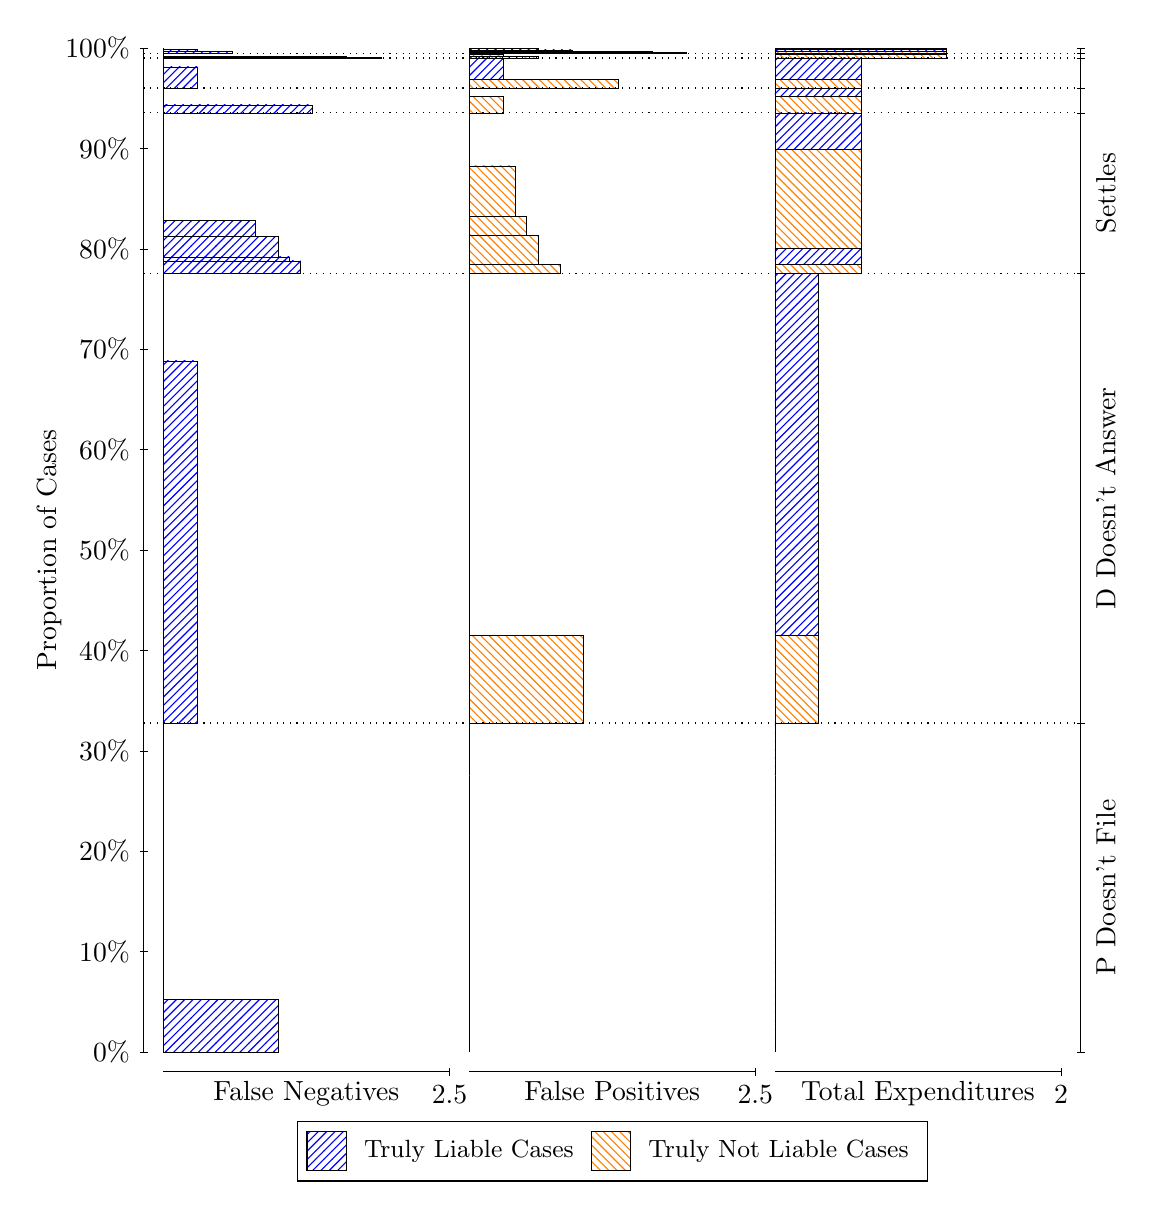
\begin{tikzpicture}
\draw[black, very thin] (1.5,1.75) -- (1.5,14.5);
\node[rotate=90, text=black, anchor=center] at (0.3, 8.125) {Proportion of Cases};
\draw[black, very thin] (1.45,1.75) -- (1.55,1.75);
\node[text=black, anchor=east] at (1.45, 1.75) {0\%};
\draw[black, very thin] (1.45,3.025) -- (1.55,3.025);
\node[text=black, anchor=east] at (1.45, 3.025) {10\%};
\draw[black, very thin] (1.45,4.3) -- (1.55,4.3);
\node[text=black, anchor=east] at (1.45, 4.3) {20\%};
\draw[black, very thin] (1.45,5.575) -- (1.55,5.575);
\node[text=black, anchor=east] at (1.45, 5.575) {30\%};
\draw[black, very thin] (1.45,6.85) -- (1.55,6.85);
\node[text=black, anchor=east] at (1.45, 6.85) {40\%};
\draw[black, very thin] (1.45,8.125) -- (1.55,8.125);
\node[text=black, anchor=east] at (1.45, 8.125) {50\%};
\draw[black, very thin] (1.45,9.4) -- (1.55,9.4);
\node[text=black, anchor=east] at (1.45, 9.4) {60\%};
\draw[black, very thin] (1.45,10.675) -- (1.55,10.675);
\node[text=black, anchor=east] at (1.45, 10.675) {70\%};
\draw[black, very thin] (1.45,11.95) -- (1.55,11.95);
\node[text=black, anchor=east] at (1.45, 11.95) {80\%};
\draw[black, very thin] (1.45,13.225) -- (1.55,13.225);
\node[text=black, anchor=east] at (1.45, 13.225) {90\%};
\draw[black, very thin] (1.45,14.5) -- (1.55,14.5);
\node[text=black, anchor=east] at (1.45, 14.5) {100\%};

\draw[black, very thin] (13.4,1.75) -- (13.4,14.5);
\draw[black, very thin] (13.35,1.75) -- (13.45,1.75);
\node[anchor=west] at (13.35, 1.75) {};
\draw[black, very thin] (13.35,5.9277) -- (13.45,5.9277);
\node[anchor=west] at (13.35, 5.9277) {};
\draw[black, very thin] (13.35,11.64) -- (13.45,11.64);
\node[anchor=west] at (13.35, 11.64) {};
\draw[black, very thin] (13.35,13.676) -- (13.45,13.676);
\node[anchor=west] at (13.35, 13.676) {};
\draw[black, very thin] (13.35,13.992) -- (13.45,13.992);
\node[anchor=west] at (13.35, 13.992) {};
\draw[black, very thin] (13.35,14.374) -- (13.45,14.374);
\node[anchor=west] at (13.35, 14.374) {};
\draw[black, very thin] (13.35,14.436) -- (13.45,14.436);
\node[anchor=west] at (13.35, 14.436) {};
\draw[black, very thin] (13.35,14.5) -- (13.45,14.5);
\node[anchor=west] at (13.35, 14.5) {};

\draw[black, very thin, pattern color=blue, pattern=north east lines] (1.75,1.75) rectangle (3.2033,2.4162);
\draw[black, very thin, pattern color=orange, pattern=north west lines] (1.75,2.4162) rectangle (1.75,5.9277);
\draw[black, very thin, pattern color=blue, pattern=north east lines] (1.75,5.9277) rectangle (2.186,10.528);
\draw[black, very thin, pattern color=orange, pattern=north west lines] (1.75,10.528) rectangle (1.75,11.64);
\draw[black, very thin, pattern color=blue, pattern=north east lines] (1.75,11.64) rectangle (3.494,11.796);
\draw[black, very thin, pattern color=blue, pattern=north east lines] (1.75,11.796) rectangle (3.3487,11.848);
\draw[black, very thin, pattern color=blue, pattern=north east lines] (1.75,11.848) rectangle (3.2033,12.107);
\draw[black, very thin, pattern color=blue, pattern=north east lines] (1.75,12.107) rectangle (2.9127,12.314);
\draw[black, very thin, pattern color=orange, pattern=north west lines] (1.75,12.314) rectangle (1.75,13.676);
\draw[black, very thin, pattern color=blue, pattern=north east lines] (1.75,13.676) rectangle (3.6393,13.779);
\draw[black, very thin, pattern color=orange, pattern=north west lines] (1.75,13.779) rectangle (1.75,13.992);
\draw[black, very thin, pattern color=blue, pattern=north east lines] (1.75,13.992) rectangle (2.186,14.26);
\draw[black, very thin, pattern color=orange, pattern=north west lines] (1.75,14.26) rectangle (1.75,14.374);
\draw[black, very thin, pattern color=blue, pattern=north east lines] (1.75,14.374) rectangle (4.5113,14.379);
\draw[black, very thin, pattern color=blue, pattern=north east lines] (1.75,14.379) rectangle (4.0753,14.395);
\draw[black, very thin, pattern color=orange, pattern=north west lines] (1.75,14.395) rectangle (1.75,14.436);
\draw[black, very thin, pattern color=blue, pattern=north east lines] (1.75,14.436) rectangle (2.622,14.461);
\draw[black, very thin, pattern color=blue, pattern=north east lines] (1.75,14.461) rectangle (2.186,14.479);
\draw[black, very thin, pattern color=orange, pattern=north west lines] (1.75,14.479) rectangle (1.75,14.5);
\draw[black, very thin, pattern color=orange, pattern=north west lines] (5.6333,1.75) rectangle (5.6333,5.2615);
\draw[black, very thin, pattern color=blue, pattern=north east lines] (5.6333,5.2615) rectangle (5.6333,5.9277);
\draw[black, very thin, pattern color=orange, pattern=north west lines] (5.6333,5.9277) rectangle (7.0867,7.0395);
\draw[black, very thin, pattern color=blue, pattern=north east lines] (5.6333,7.0395) rectangle (5.6333,11.64);
\draw[black, very thin, pattern color=orange, pattern=north west lines] (5.6333,11.64) rectangle (6.796,11.751);
\draw[black, very thin, pattern color=orange, pattern=north west lines] (5.6333,11.751) rectangle (6.5053,12.116);
\draw[black, very thin, pattern color=orange, pattern=north west lines] (5.6333,12.116) rectangle (6.36,12.363);
\draw[black, very thin, pattern color=orange, pattern=north west lines] (5.6333,12.363) rectangle (6.2147,13.003);
\draw[black, very thin, pattern color=blue, pattern=north east lines] (5.6333,13.003) rectangle (5.6333,13.676);
\draw[black, very thin, pattern color=orange, pattern=north west lines] (5.6333,13.676) rectangle (6.0693,13.889);
\draw[black, very thin, pattern color=blue, pattern=north east lines] (5.6333,13.889) rectangle (5.6333,13.992);
\draw[black, very thin, pattern color=orange, pattern=north west lines] (5.6333,13.992) rectangle (7.5227,14.106);
\draw[black, very thin, pattern color=blue, pattern=north east lines] (5.6333,14.106) rectangle (6.0693,14.374);
\draw[black, very thin, pattern color=orange, pattern=north west lines] (5.6333,14.374) rectangle (6.5053,14.398);
\draw[black, very thin, pattern color=orange, pattern=north west lines] (5.6333,14.398) rectangle (6.0693,14.415);
\draw[black, very thin, pattern color=blue, pattern=north east lines] (5.6333,14.415) rectangle (5.6333,14.436);
\draw[black, very thin, pattern color=orange, pattern=north west lines] (5.6333,14.436) rectangle (8.3947,14.441);
\draw[black, very thin, pattern color=orange, pattern=north west lines] (5.6333,14.441) rectangle (7.9587,14.457);
\draw[black, very thin, pattern color=blue, pattern=north east lines] (5.6333,14.457) rectangle (6.9413,14.475);
\draw[black, very thin, pattern color=blue, pattern=north east lines] (5.6333,14.475) rectangle (6.5053,14.5);
\draw[black, very thin, pattern color=orange, pattern=north west lines] (9.5167,1.75) rectangle (9.5167,5.2615);
\draw[black, very thin, pattern color=blue, pattern=north east lines] (9.5167,5.2615) rectangle (9.5167,5.9277);
\draw[black, very thin, pattern color=orange, pattern=north west lines] (9.5167,5.9277) rectangle (10.062,7.0395);
\draw[black, very thin, pattern color=blue, pattern=north east lines] (9.5167,7.0395) rectangle (10.062,11.64);
\draw[black, very thin, pattern color=orange, pattern=north west lines] (9.5167,11.64) rectangle (10.607,11.751);
\draw[black, very thin, pattern color=blue, pattern=north east lines] (9.5167,11.751) rectangle (10.607,11.957);
\draw[black, very thin, pattern color=orange, pattern=north west lines] (9.5167,11.957) rectangle (10.607,13.209);
\draw[black, very thin, pattern color=blue, pattern=north east lines] (9.5167,13.209) rectangle (10.607,13.676);
\draw[black, very thin, pattern color=orange, pattern=north west lines] (9.5167,13.676) rectangle (10.607,13.889);
\draw[black, very thin, pattern color=blue, pattern=north east lines] (9.5167,13.889) rectangle (10.607,13.992);
\draw[black, very thin, pattern color=orange, pattern=north west lines] (9.5167,13.992) rectangle (10.607,14.106);
\draw[black, very thin, pattern color=blue, pattern=north east lines] (9.5167,14.106) rectangle (10.607,14.374);
\draw[black, very thin, pattern color=orange, pattern=north west lines] (9.5167,14.374) rectangle (11.697,14.415);
\draw[black, very thin, pattern color=blue, pattern=north east lines] (9.5167,14.415) rectangle (11.697,14.436);
\draw[black, very thin, pattern color=orange, pattern=north west lines] (9.5167,14.436) rectangle (11.697,14.453);
\draw[black, very thin, pattern color=blue, pattern=north east lines] (9.5167,14.453) rectangle (11.697,14.478);
\draw[black, very thin, pattern color=orange, pattern=north west lines] (9.5167,14.478) rectangle (11.697,14.483);
\draw[black, very thin, pattern color=blue, pattern=north east lines] (9.5167,14.483) rectangle (11.697,14.5);
\draw[black, dotted] (1.5,5.9277) -- (13.4,5.9277);
\draw[black, dotted] (1.5,11.64) -- (13.4,11.64);
\draw[black, dotted] (1.5,13.676) -- (13.4,13.676);
\draw[black, dotted] (1.5,13.992) -- (13.4,13.992);
\draw[black, dotted] (1.5,14.374) -- (13.4,14.374);
\draw[black, dotted] (1.5,14.436) -- (13.4,14.436);
\draw[black, very thin] (1.75,1.5) -- (5.3833,1.5);
\node[text=black, anchor=north] at (3.5667, 1.5) {False Negatives};
\draw[black, very thin] (5.3833,1.45) -- (5.3833,1.55);
\node[text=black, anchor=north] at (5.3833, 1.45) {2.5};

\draw[black, very thin] (5.6333,1.5) -- (9.2667,1.5);
\node[text=black, anchor=north] at (7.45, 1.5) {False Positives};
\draw[black, very thin] (9.2667,1.45) -- (9.2667,1.55);
\node[text=black, anchor=north] at (9.2667, 1.45) {2.5};

\draw[black, very thin] (9.5167,1.5) -- (13.15,1.5);
\node[text=black, anchor=north] at (11.333, 1.5) {Total Expenditures};
\draw[black, very thin] (13.15,1.45) -- (13.15,1.55);
\node[text=black, anchor=north] at (13.15, 1.45) {2};

\node[text=black, centered, rotate=90] at (13.72, 3.8389) {P Doesn't File};
\node[text=black, centered, rotate=90] at (13.72, 8.7839) {D Doesn't Answer};
\node[text=black, centered, rotate=90] at (13.72, 12.658) {Settles};





\draw (7.449999999999999,1.5) node[draw=none] (baseCoordinate) {};
\begin{scope}[align=center]
        \matrix[scale=0.5, draw=black, below=0.5cm of baseCoordinate, nodes={draw}, column sep=0.1cm]{
            \node[rectangle, draw, minimum width=0.5cm, minimum height=0.5cm, pattern color=blue, pattern=north east lines] {}; &
            \node[draw=none, font=\small, text=black] (B) {Truly Liable Cases}; &
            \node[rectangle, draw, minimum width=0.5cm, minimum height=0.5cm, pattern color=orange, pattern=north west lines] {}; &
            \node[draw=none, font=\small, text=black] (B) {Truly Not Liable Cases}; \\
            };
\end{scope}

\end{tikzpicture}
\end{document}